\documentclass[t,12pt,numbers,fleqn,usenames,xcolor=dvipsnames]{beamer}
%\documentclass[t,12pt,numbers,fleqn,handout]{beamer}

\usepackage{amsmath}
\usepackage{mathtools}
\usepackage{amsfonts}
\usepackage{paralist}
\usepackage{latexsym}
\usepackage{amssymb}
\usepackage{stmaryrd}
\usepackage{phonetic}
\usepackage{wasysym}
\usepackage{pgf}
\usepackage{tikz}
\usepackage{url}
\usetikzlibrary{arrows}
\usepackage{array}
\usepackage{pgfpages} 
\usepackage{multirow} 
\usepackage{graphicx}
\usepackage{color}
\usepackage{listings,lstautogobble}
\lstset{
	basicstyle=\ttfamily,
	mathescape
}
\usepackage{calc}
\usepackage{tikz}
\usepackage{tikz-cd}
\usetikzlibrary{tikzmark,calc,decorations.pathreplacing,positioning,fadings}
\usepackage{hyperref}
\usepackage{verbatim}
\usepackage{fancyvrb}
\usepackage{tabularx}
\usepackage{tikz}
\usepackage{tikz-cd}
\usetikzlibrary{cd}
\usepackage{graphicx}
\usepackage{collectbox}
\usepackage{tabularx}
\usepackage{wrapfig}
\usepackage{lscape}
\usepackage{textcomp}
\usepackage[show]{ed}
\usepackage{adjustbox}
\setlength{\arrayrulewidth}{1mm}
\setlength{\tabcolsep}{18pt}
\renewcommand{\arraystretch}{1.5}
\hypersetup{colorlinks=true,
    linkcolor=blue,
    citecolor=blue,
    filecolor=blue,
    urlcolor=blue,
    unicode=false}

\usepackage{macros/myMacros}
\usepackage{macros/local}
\usepackage{macros/basics}

% To include lagda 
%\usepackage{latex/agda}
%\usepackage{ucs}
%\usepackage[utf8x]{inputenc}
%\usepackage{autofe}
%\usepackage{fancyvrb}
%\DefineVerbatimEnvironment
%{code}{Verbatim}


\lstset{language=lisp,basicstyle=\ttfamily,breaklines=true,showspaces=false,showstringspaces=false,breakatwhitespace=true,texcl=true,escapeinside={\%*}{*)}}
\tikzstyle{stuff_fill}=[rectangle,draw,fill=black!20,minimum size=1.4em]


\usepackage{fancybox}

\mode<presentation>{}


\usetheme{default}
\setbeamertemplate{navigation symbols}{} 
\setbeamertemplate{itemize item}[ball]
\setbeamersize{text margin left = 4mm}
\setbeamersize{text margin right = 4mm}

%\input{def-beamer}

\title{Diagram Combinators in MMT}
\subtitle{Modular Building of Large Libraries}
\author{Florian Rabe$^1$ and \underline{Yasmine Sharoda$^2$}}
\institute{$^1$FAU Erlangen-N{\"u}rnberg, Germany and LRI, Universit{\'e} Paris Sud, France  \and
	$^2$ McMaster University, Canada}
\date{}
	
\newcommand\textline[4][t]{%
	\par\smallskip\noindent\parbox[#1]{.333\textwidth}{\raggedright\texttt{+}#2}%
	\parbox[#1]{.333\textwidth}{\centering#3}%
	\parbox[#1]{.333\textwidth}{\raggedleft\texttt{#4}}\par\smallskip%
}	

\setbeamertemplate{footline}[frame number]

\newcommand{\icsg}{\cn{IdempotentCommutativeSemigroup}\xspace}
	
\begin{document}

\begin{frame}

\titlepage


\end{frame}

\begin{frame}{Table of Contents}
\tableofcontents
\end{frame}

\section{Motivation}
\begin{frame}[fragile]{Motivation}
Building the algebraic hierarchy 
\begin{itemize}
	\item[] From: \Magma \verb|(U,*)|
	\item[] To \icsg 
\end{itemize}
\begin{onlyenv}<1>
\scriptsize{
\begin{center}
	\begin{tikzpicture}[scale=.8]
	\node (M)    at (0,0)      {\Magma};
	\node (CM) at (-4,-1) {\CommMagma};
	\node (SG)  at (0,-1)   {\Semigroup};
	\node (IM)  at  (4,-1)   {\IdempMagma};
	\draw[mono](M) -- (CM);
	\draw[mono](M) -- (SG); 
	\draw[mono](M) -- (IM);
	\node (CSG)  at (-5,-2)   {\CommutativeSemigroup};
	\node (ISG)    at (5,-2)    {\IdempotentSemigroup};
	\node (ICM)    at (0,-2)    {\IdempotentCommutativeMagma};
	\node (ACSG)  at (0,-3)   {\IdempotentCommutativeSemigroup};
	\draw[mono](CM) -- (CSG);
	\draw[mono](CM) -- (ICM);
	\draw[mono](IM) -- (ISG); 
	\draw[mono](IM) -- (ICM);
	\draw[mono](SG) -- (ISG); 
	\draw[mono](SG) -- (CSG);
	\draw[mono](CSG) -- (ACSG);
	\draw[mono](ISG) -- (ACSG);
	\draw[mono](ICM) -- (ACSG);
	\end{tikzpicture}
\end{center}}
\end{onlyenv}
\begin{onlyenv}<2>
\begin{enumerate}
	\item[1.] Flat Theories 
\scriptsize{
	\begin{lstlisting}
Theory $\icsg$ := {
  U : type 
  $\_\circ\_$ : U $\rightarrow$ U $\rightarrow$ U 
  associativity : $\cdots$
  commutativity : $\cdots$
  idempotence : $\cdots$
  }
	\end{lstlisting}}
\scriptsize{
\begin{center}
		\begin{tikzpicture}[scale=.8]
		\node (M)    at (0,0)      {\Magma};
		\node (CM) at (-4,-1) {\CommMagma};
		\node (SG)  at (0,-1)   {\Semigroup};
		\node (IM)  at  (4,-1)   {\IdempMagma};
		\node (CSG)  at (-5,-2)   {\CommutativeSemigroup};
		\node (ISG)    at (5,-2)    {\IdempotentSemigroup};
		\node (ICM)    at (0,-2)    {\IdempotentCommutativeMagma};
		\node (ACSG)  at (0,-3)   {\IdempotentCommutativeSemigroup};
		\end{tikzpicture}
\end{center}}
\end{enumerate}
\end{onlyenv}
\begin{onlyenv}<3>
\begin{enumerate}
	\item[2.] Theory Formation Operators 
	\begin{itemize}
		\item Extension 
		\item Colimit
	\end{itemize}
\end{enumerate}
\end{onlyenv}
\begin{onlyenv}<4>
	\scriptsize{
\begin{lstlisting}
IdempotentMagma := Magma extended_by {idemp : }
CommutativeMagma := Magma extended_by {comm : }
Semigroup := Magma extended_by {assoc : }
\end{lstlisting}}
\scriptsize{
	\begin{center}
		\begin{tikzpicture}[scale=.8]
		\node (M)    at (0,0)      {\Magma};
		\node (CM) at (-4,-1) {\CommMagma};
		\node (SG)  at (0,-1)   {\Semigroup};
		\node (IM)  at  (4,-1)   {\IdempMagma};
		\draw[mono](M) -- (CM);
		\draw[mono](M) -- (SG); 
		\draw[mono](M) -- (IM);
		\end{tikzpicture}
\end{center}}
\end{onlyenv}
\begin{onlyenv}<5>
	\scriptsize{
		\begin{lstlisting}
IdempotentMagma := Magma extended_by {idemp : }
CommutativeMagma := Magma extended_by {comm : }
Semigroup := Magma extended_by {assoc : }
IdempotentSemigroup := Combine IdempotentMagma Semigroup
CommutativeSemigroup := Combine CommutativeMagma Semigroup 
IdempotentCommutative := 
Combine IdempotentMagma CommutativeMagma 
IdempotentCommutativeSemigroup := 
Combine IdempotentMagma CommutativeMagma Semigroup
		\end{lstlisting}}
	\scriptsize{
		\begin{center}
			\begin{tikzpicture}[scale=.8]
			\node (M)    at (0,0)      {\Magma};
			\node (CM) at (-4,-1) {\CommMagma};
			\node (SG)  at (0,-1)   {\Semigroup};
			\node (IM)  at  (4,-1)   {\IdempMagma};
			\draw[mono](M) -- (CM);
			\draw[mono](M) -- (SG); 
			\draw[mono](M) -- (IM);
			\node (CSG)  at (-5,-2)   {\CommutativeSemigroup};
			\node (ISG)    at (5,-2)    {\IdempotentSemigroup};
			\node (ICM)    at (0,-2)    {\IdempotentCommutativeMagma};
			\node (ACSG)  at (0,-3)   {\IdempotentCommutativeSemigroup};
			\draw[mono](CM) -- (CSG);
			\draw[mono](CM) -- (ICM);
			\draw[mono](IM) -- (ISG); 
			\draw[mono](IM) -- (ICM);
			\draw[mono](SG) -- (ISG); 
			\draw[mono](SG) -- (CSG);
			\draw[mono](CSG) -- (ACSG);
			\draw[mono](ISG) -- (ACSG);
			\draw[mono](ICM) -- (ACSG);
			\end{tikzpicture}
	\end{center}}
\pause
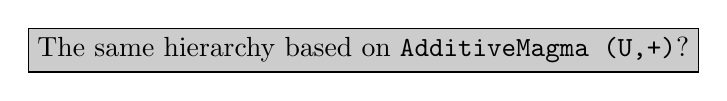
\begin{tikzpicture}
\draw (1,1) node [stuff_fill] {The same hierarchy based on \verb|AdditiveMagma (U,+)|?};
\end{tikzpicture}
\end{onlyenv}
\begin{onlyenv}<6>
\begin{enumerate}
	\item[3.] Diagram Formation Operators  
\scriptsize{
		\begin{lstlisting}
IdempotentMagma := Magma extended_by {idemp : }
CommutativeMagma := Magma extended_by {comm : }
Semigroup := Magma extended_by {assoc : }
IdempotentCommutativeSemigroup := 
 BCOMBINE (diag (IdempotentMagma CommutativeMagma Semigroup))
	\end{lstlisting}}
	\scriptsize{
	\begin{center}
		\begin{tikzpicture}[scale=.8]
		\node (M)    at (0,0)      {\Magma};
		\node (CM) at (-4,-1) {\CommMagma};
		\node (SG)  at (0,-1)   {\Semigroup};
		\node (IM)  at  (4,-1)   {\IdempMagma};
		\draw[mono](M) -- (CM);
		\draw[mono](M) -- (SG); 
		\draw[mono](M) -- (IM);
		\node (CSG)  at (-5,-2)   {\CommutativeSemigroup};
		\node (ISG)    at (5,-2)    {\IdempotentSemigroup};
		\node (ICM)    at (0,-2)    {\IdempotentCommutativeMagma};
		\node (ACSG)  at (0,-3)   {\IdempotentCommutativeSemigroup};
		\draw[mono](CM) -- (CSG);
		\draw[mono](CM) -- (ICM);
		\draw[mono](IM) -- (ISG); 
		\draw[mono](IM) -- (ICM);
		\draw[mono](SG) -- (ISG); 
		\draw[mono](SG) -- (CSG);
		\draw[mono](CSG) -- (ACSG);
		\draw[mono](ISG) -- (ACSG);
		\draw[mono](ICM) -- (ACSG);
		\end{tikzpicture}
\end{center}}
\end{enumerate}
\end{onlyenv}
\end{frame}

\section{Contribution}
\begin{frame}[fragile]{Contribution}
Formal language for creating and manipulating diagrams. 
\begin{itemize}
	\item Operations Implemented in MMT 
	\item Extensible environment to allow user defined operations 
\end{itemize}
\end{frame}

\begin{frame}[fragile]{Diagram: Definition}
A \textbf{diagram} $D$ consists of
\begin{itemize}
	\item a list of \textbf{nodes}: \node{l}{D(l)} 
	\item a list of \textbf{edges}, each written as \edge{l}{d}{c}{D(l)} 
	\item an optional label $\dist{D}$ of a node --- the \textbf{distinguished} node
	\item an optional label $\iedge{l}{d}{c}{D(l)}$ of an arrow -- the \textbf{implicit} arrow 
\end{itemize}
\end{frame}

\begin{frame}[fragile]{Diagram: Examples}
\scriptsize{
	\begin{lstlisting}
diagram Semigroup := Magma extended_by {associativity : $\cdots$}
diagram CommutativeMagma := Magma extended_by {commutativity : $\cdots$}
	\end{lstlisting}}
\begin{center}
\begin{tikzcd}
	Magma \arrow[r,blue] & \textcolor{blue}{\cn{Semigroup}} \\ 
	Magma \arrow[r,blue] & \textcolor{blue}{\cn{CommutativeMagma}}	
\end{tikzcd} 
\end{center}
\scriptsize{
	\begin{lstlisting}
diagram PointedMagma := Combine Semigroup CommutativeMagma
	\end{lstlisting}}
\begin{tikzcd}
	Magma \arrow[r] \arrow[d] \arrow[rd,blue]
	& Semigroup \arrow[d]  \\
	CommutativeMagma \arrow[r] & \textcolor{blue}{\cn{CommutativeSemigroup}}
\end{tikzcd} 
\end{frame}


\begin{frame}[fragile]{Building tiny diagrams}
Interpreting combinators from CITATION as diagram operations 
\begin{onlyenv}<1>
\begin{enumerate}
\item[1.] Extension 
\begin{lstlisting}
diagram d$^{\prime}$ := d extended_by $\Sigma$ 
\end{lstlisting}
\begin{columns}
	\begin{column}{0.45\textwidth}
Input Diagram: \\
\begin{tikzcd}
	\arrow[r] & \dist{D}  
\end{tikzcd} 
	\end{column}
	\begin{column}{0.45\textwidth}
Output Diagram: 
\begin{tikzcd}
	\arrow[r] & \dist{D} \arrow[r,,blue] & \textcolor{blue}{\pres} \\%\dist{D} \rtimes \Sigma}  \\
\end{tikzcd} 
\end{column}
\end{columns}
Example: 
\end{enumerate}
\end{onlyenv}

\begin{onlyenv}<2>
\begin{enumerate}
	\item[2.] Rename 	
	\begin{lstlisting}
diagram d$^{\prime}$ := d rename r 
	\end{lstlisting}
	\begin{columns}
		\begin{column}{0.45\textwidth}
			Input Diagram: \\
\begin{tikzcd}
	\arrow[r] & \dist{D} \\
\end{tikzcd} 
		\end{column}
		\begin{column}{0.45\textwidth}
			Output Diagram: 
\begin{tikzcd}
	\arrow[r] & \dist{D}  \arrow[r,,blue] & \textcolor{blue}{\pres} \\%r \cdot \dist{D}}  \\
\end{tikzcd} 
		\end{column}
	\end{columns}
	Example: 
\end{enumerate}	
\end{onlyenv}

\begin{onlyenv}<3>
	\begin{enumerate}
		\item[3.] Combine 	
		\begin{lstlisting}
diagram d$^{\prime}$ := combine d$_1$ r$_1$ d$_2$ r$_2$ 
		\end{lstlisting}
		\begin{columns}
			\begin{column}{0.45\textwidth}
				Input Diagram: \\
\scriptsize{				
\begin{tikzcd}
	S \arrow[r] \arrow[d]
	& \dist{D_1}  \\
	\dist{D_2}
	% \arrow[red]{r}[blue]{\eta}
\end{tikzcd}}
			\end{column}
			\begin{column}{0.45\textwidth}
				Output Diagram: 
\scriptsize{
\begin{tikzcd}
	S \arrow[r] \arrow[d] \arrow[rdrd,blue]
	& \dist{D_1} \arrow[r] & \dist{D_1} \cdot r_1 \arrow[dd] \\
	\dist{D_2} \arrow[d] \\ 
	\dist{D_2} \cdot r_2 \arrow[rr] && \textcolor{blue}{\cn{pres}}
\end{tikzcd} }
			\end{column}
		\end{columns}
		Example: 
	\end{enumerate}	
\end{onlyenv}

\begin{onlyenv}<4>
	\begin{enumerate}
		\item[3.] Mixin 	
		\begin{lstlisting}
		diagram d$^{\prime}$ := diagram d rename r 
		\end{lstlisting}
		\begin{columns}
			\begin{column}{0.45\textwidth}
				Input Diagram: \\
				\begin{tikzcd}
					\arrow[r] & \dist{D} \\
				\end{tikzcd} 
			\end{column}
			\begin{column}{0.45\textwidth}
				Output Diagram: 
				\begin{tikzcd}
					\arrow[r] & \dist{D}  \arrow[r,,blue] & \textcolor{blue}{\pres} \\%r \cdot \dist{D}}  \\
				\end{tikzcd} 
			\end{column}
		\end{columns}
		Example: 
	\end{enumerate}	
\end{onlyenv}
%\input{table}
\end{frame}

\begin{frame}[fragile]{Building Bigger Diagrams}
\begin{itemize}
	\item Using names  
	\item Set theoretic Operations 
\end{itemize}
\end{frame}

\begin{frame}[fragile]{Even Bigger Diagrams: Batch Operations}
\begin{itemize}
	\item Batch Combine 
	\item Batch Mixin 
\end{itemize}
\end{frame}

\begin{frame}[fragile]{Choosing Names}
show an example 
\end{frame}

\section{Realization}
\begin{frame}[fragile]{Extensible Environment}
\begin{itemize}
	\item Define a new MMT theory 
	\item Define a scala rule for computing the output diagram via manipulating omDoc terms p
\end{itemize}
\end{frame}

\end{document}
